\section{Results}
\label{sec:results}
Unless specified otherwise, numerical examples below use the heterogeneous mechanism, $n=499$, and pointwise 95\% intervals across independent full-dataset repetitions. They illustrate prespecified comparisons; all dimensions, calibration sizes, scenarios and environments remain in the delivered cell summaries. An interval near nominal is not an equivalence test or proof of exact validity.

\begin{table}[t]
\centering
\caption[Main reliability and area comparison]{\textbf{Reliability and common area in the heterogeneous $K=3$ setting.} Calibration size is 499; entries show replication means $\pm$ pointwise 95\% interval half-widths, not standard deviations across runs. The shifted group-1 probability is 0.8 versus 0.2 for iid evaluation. Area is a fraction of Euclidean simplex area, averaged over iid feature anchors. Smaller area is useful only with adequate coverage; coordinatewise naive is the negative control. TV exactly duplicates raw maximum at $K=3$; forward KL uses $y\Vert\hat\mu$. These intervals are not simultaneous. Full-cell estimates and replication counts are supplied in \texttt{tables/all\_estimates.csv}.
}
\label{tab:main}
{\small\begin{tabular}{lrrrr}
\toprule
Method & \shortstack{Joint\\iid} & \shortstack{Group 1\\iid} & \shortstack{Joint\\shifted} & \shortstack{Area fraction\\iid} \\
\midrule
Raw Euclidean & $0.902\pm0.003$ & $0.512\pm0.013$ & $0.608\pm0.010$ & $0.232\pm0.010$ \\
Raw maximum & $0.902\pm0.003$ & $0.512\pm0.013$ & $0.609\pm0.010$ & $0.230\pm0.010$ \\
Total variation & $0.902\pm0.003$ & $0.512\pm0.013$ & $0.609\pm0.010$ & $0.230\pm0.010$ \\
Forward KL & $0.902\pm0.003$ & $0.511\pm0.012$ & $0.608\pm0.010$ & $0.216\pm0.008$ \\
Aitchison & $0.902\pm0.003$ & $0.507\pm0.014$ & $0.605\pm0.011$ & $0.253\pm0.010$ \\
Scaled Aitchison & $0.901\pm0.003$ & $0.899\pm0.005$ & $0.898\pm0.004$ & $0.157\pm0.008$ \\
Group Aitchison & $0.903\pm0.003$ & $0.906\pm0.005$ & $0.905\pm0.004$ & $0.164\pm0.008$ \\
Oracle weighted & $0.902\pm0.003$ & $0.507\pm0.014$ & $0.907\pm0.005$ & $0.253\pm0.010$ \\
Coord. naive & $0.839\pm0.003$ & $0.324\pm0.007$ & $0.451\pm0.006$ & $0.090\pm0.003$ \\
Coord. Bonferroni & $0.936\pm0.002$ & $0.681\pm0.009$ & $0.744\pm0.008$ & $0.317\pm0.009$ \\
\bottomrule
\end{tabular}
}
\end{table}
\begin{figure}[t]
\centering
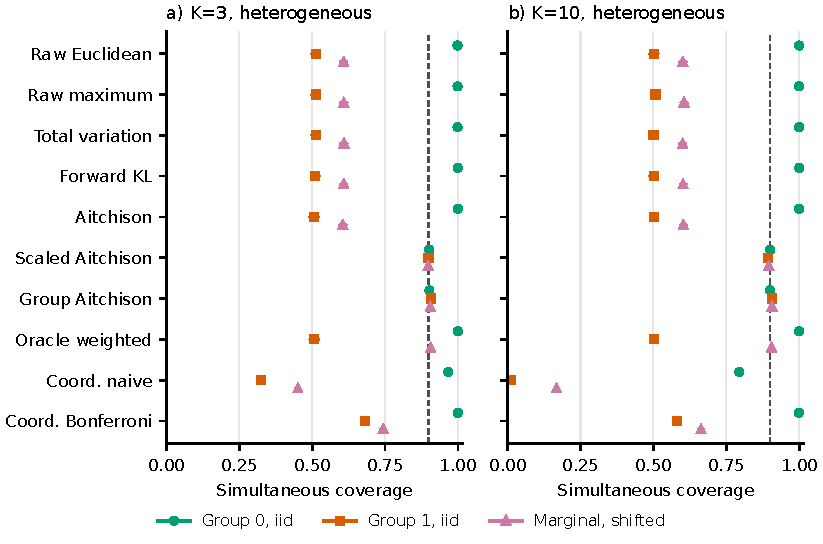
\includegraphics[width=\linewidth]{figures/group_shift_coverage.pdf}
\caption[Subgroups and mixture shift]{\textbf{Subgroup coverage and controlled mixture shift.} Dots are means across 100 independent train/calibration/test replications; bars are pointwise 95\% $t$ intervals for these means, not simultaneous bands or intervals for a single calibrated run. Each replication uses 1000 training and 499 calibration observations and 5000 test observations per environment. Circles and squares are iid coverage in the prespecified lower-noise group 0 and higher-noise group 1. Triangles are marginal coverage after the test group-1 probability changes from $0.2$ to $0.8$, with within-group laws preserved. Colors and shapes distinguish estimands; shifted marginal coverage is not a third subgroup. ``Group Aitchison'' calibrates within observed groups; ``Oracle weighted'' uses the known density ratio, unavailable in general applications. The dashed line marks 0.90. TV exactly duplicates raw maximum at $K=3$; KL is forward $y\Vert\hat\mu$. This experiment does not test arbitrary shift.
}
\label{fig:groups}
\end{figure}
\paragraph{Joint calibration is necessary for joint reliability.}
At $K=3$, iid joint coverage is $\NaiveJoint{}$ for naive coordinate calibration, $\BonfJoint{}$ for Bonferroni, $\RawJoint{}$ for raw L2 and $\GlobalJoint{}$ for global Aitchison. The naive control falls to $\NaiveTen{}$ at $K=10$. Thus coordinatewise calibration can fail substantially at the vector level, despite each coordinate being calibrated separately. Bonferroni is a valid but conservative control. Joint-score iid marginal means across the core matrix remain close to their rank targets; this does not mean every individual pointwise interval contains $0.9$ or that regions have equal size.

\paragraph{Marginal success conceals subgroup failure.}
For global Aitchison at $K=3$, low-noise-group coverage is $\GlobalLow{}$ while high-noise-group coverage is $\GlobalHigh{}$. Their mixture produces acceptable marginal coverage while allocating misses very unevenly (Figure~\ref{fig:groups}; Table~\ref{tab:main}). Mondrian calibration gives low/high group coverages $\GroupLow{}$ and $\GroupHigh{}$; learned scaling gives $\ScaledLow{}$ and $\ScaledHigh{}$. Both adapt strongly in this mechanism. The negative result matters: at $K=10$, scaled high-noise-group coverage is $\ScaledTenHigh{}$, below nominal in this pointwise estimate. A learned scale is useful here without acquiring a distribution-free group guarantee.

\paragraph{Geometry and adaptation change measured area.}
At $K=3$, mean iid Euclidean simplex-area fractions are $\GlobalArea{}$ for global Aitchison, $\RawArea{}$ for raw L2 and $\MaxArea{}$ for raw max. Scaling and Mondrian give $\ScaledArea{}$ and $\GroupArea{}$. Their paired area differences from global Aitchison are $\ScaledAreaDiff{}$ and $\GroupAreaDiff{}$. Figure~\ref{fig:area} puts these areas beside the homogeneous comparison. These results support a smaller expected area for adaptive regions in this iid heterogeneous setting, with coverage shown alongside size. They do not make raw/global regions group-valid, establish a measure-independent ranking or transfer to $K=10$. Some other prespecified area contrasts remain unresolved, including raw L2/max versus global Aitchison under heterogeneous shift at $n=99$ and scaled versus global Aitchison under homogeneous shift. We withhold their orderings.

\paragraph{Prior-work scores do not remove the diagnostic failures.}
The source-driven controls give TV joint coverage $\TVJoint{}$ and forward-KL coverage $\KLJoint{}$ in the same $K=3$ iid cell. Forward-KL high-noise-group coverage is $\KLHigh{}$ and shifted marginal coverage is $\KLShift{}$. Thus changing these score geometries alone does not repair group or unweighted-shift failures. Forward-KL area is $\KLArea{}$, with paired KL-minus-raw-L2 difference $\KLRawAreaDiff{}$. This is a smaller iid area under the chosen reference, not a universal optimum. All 800 matched $K=3$ TV coverage/group/area rows exactly duplicate raw max; TV is distinct at $K=10$. Appendix Table~\ref{tab:prior_area} gives the paired area contrasts. These comparisons hold our predictor fixed rather than reproduce a prior study's complete fitted pipeline.

\begin{figure}[t]
\centering
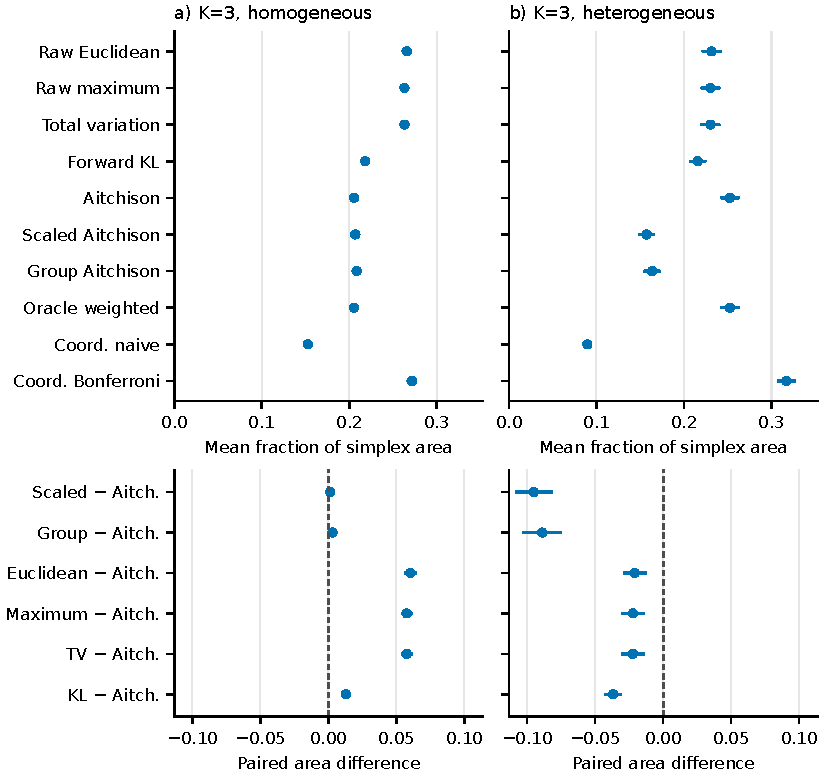
\includegraphics[width=\linewidth]{figures/simplex_area.pdf}
\caption[Common simplex area and paired differences]{\textbf{A common area measure for $K=3$.} Dots are means across 100 independent train/calibration/test replications; bars are pointwise 95\% $t$ intervals for these means, not simultaneous bands or intervals for a single calibrated run. Each replication uses 1000 training and 499 calibration observations and 5000 test observations per environment. Area uses 32 independent feature anchors and 8192 common uniform-simplex candidates per anchor in each replication/environment. Top: mean fraction of Euclidean simplex area under iid sampling. The uniform-simplex reference measure is shared across methods; it is not clr volume or application utility. Bottom: paired within-replication differences from unscaled Aitchison, with pointwise 95\% $t$ intervals; negative values indicate smaller area. Interpret area jointly with the coverage displays; the naive control has no nominal joint-coverage guarantee. TV exactly duplicates raw maximum at $K=3$, so these rows are one geometry. KL is forward $y\Vert\hat\mu$. Intervals crossing zero leave area orderings unresolved. No cross-geometry size comparison is made at $K=10$.
}
\label{fig:area}
\end{figure}
\paragraph{The controlled shift exposes the hidden misses.}
At $K=3$, changing the high-noise-group frequency to $0.8$ reduces global Aitchison marginal coverage to $\GlobalShift{}$, a paired shifted-minus-iid difference of $\GlobalShiftDiff{}$. The group-mixture identity in Appendix~\ref{app:theory} explains the direction and scale of this failure. Mondrian reaches $\GroupShift{}$, oracle known-ratio weighting $\WeightedShift{}$ and learned scaling $\ScaledShift{}$. Oracle high-noise-group coverage is only $\WeightedShiftHigh{}$: restoring target-marginal coverage does not restore group coverage even with correct ratios.

Mondrian and oracle weighted areas under shift are $\GroupShiftArea{}$ and $\WeightedShiftArea{}$; the paired oracle-minus-Mondrian difference is $\WeightedGroupAreaDiff{}$. A small global region that severely undercovers is not a reliable efficiency winner. These comparisons exploit known groups or ratios and invariant within-group laws; they do not test unknown groups, learned ratios or arbitrary shift. Unit-weight oracle results coincide exactly with global Aitchison on all iid matched rows, verifying algorithm and stream matching rather than an independent replication of that method.

\paragraph{Mean coverage does not certify each calibration sample.}
For global Aitchison at $K=3$, iid finite-test coverage has across-repetition standard deviation $\CalSdSmall{}$ at $n=99$ and $\CalSdLarge{}$ at $n=499$. The empirical fractions below $0.85$ are $\CalTailSmall{}$ and $\CalTailLarge{}$, with Wilson intervals. Even zero observed failures has a positive upper confidence bound. These events concern finite-test estimates; they are not guarantees about population coverage conditional on every realized calibration set.

\paragraph{Zero replacement changes what is covered.}
At $K=10$ and $\epsilon=10^{-8}$, transformed-target global Aitchison coverage is $\BoundaryTransformed{}$. Testing the same transformed-calibrated region directly against original responses gives only $\BoundaryOriginal{}$, whereas separately calibrated original-target raw L2 gives $\BoundaryRaw{}$. The boundary-response frequency is $\BoundaryRate{}$. For transformed global Aitchison, the paired $10^{-2}$-minus-$10^{-8}$ coverage change is $\ReplacementDelta{}$, an unresolved mean-coverage change despite changed targets and fitted geometry. The full epsilon grid quantifies sensitivity on paired original datasets; changing $\epsilon$ changes both fitted geometry and the transformed target. The direct-original diagnostic is a different region from the explicit inverse image $C_{\rm pre}(x)=\{y:T_\epsilon(y)\in C_\epsilon(x)\}$. The latter has exactly the measured transformed membership event, so its original-response coverage and interval are also $\BoundaryTransformed{}$, including zeros. This is an identity from existing events, not a new simulation; its original-simplex area was not estimated. Censoring tests one zero mechanism.

\paragraph{Numerical checks and executed scope.}
The rank study executes all 30 declared continuous/tied-score cells, each with 20,000 trials, and compares empirical coverage/calibration variability with the exact rank and beta/discrete references. For uniform scores at $n=99$, $\alpha=0.1$, test coverage is $\RankUniform{}$ against theoretical $0.9$; at $n=9$ with tied Bernoulli scores it is $\RankTied{}$. Infinite-threshold cases return full coverage, while ties are conservative. Separate checks passed for clr/ilr equivalence, perturbation invariance, analytic simplex area, Bonferroni nesting, empty/tiny groups, weighted test atoms and finite/infinite serialization. No core, oracle or boundary repetition was excluded and no resource run failed. The resource-reported core, initial-extension and TV/KL running times were 116.110, 43.878 and 44.498 seconds, respectively, excluding startup; source hashes, timings, the pilot and the pre-main serialization correction are retained with the code. The source-to-claim map and inline-quantity extraction accompany the manuscript.
